\section{Systeme}
\subsection{Eigenschaften}
\textbf{Eingänge:} SISO (Single Input Single Output) und MIMO (Multiple Input Multiple Output) beschreiben die Eingänge zu Ausgänge.\\
\textbf{Aktive/Passiv:} Aktive weisen eigene Speisung auf; Passive nicht\\
\textbf{Kausal/Akausal:} \script{164} Kausal ist, wenn keine zukünftigen Werte des Eingangssignals $x(t)$, sondern nur Vergangene Werte betrachtet werden müssen. Akausal hängt auch von Zukünftigen WErten ab. Alle realen physikalische System sind kausal.\\
\textbf{Linear/Nicht Linear:} \script{165} Ein System ist Linear, wenn vervielfachung am Eingang dies auch am Ausgang widerspiegelt, Sinus Signale sind nur Phasenverschoben, haben aber die gleiche Frequenz. Nicht lineare Systeme haben neue Frequenzanteile.\\
\textbf{Invertierbar:} \script{173} $x^3$ ist invertierbar, $x^2$ nicht, weil es keine Umkehrfunktion gibt. \\
\textbf{Statische/Dynamisch:} \script{162}Statisch, der Ausgange hat nur mit dem aktuellen Eingang zu tun. Dynamisch, der Ausgang hat mit Eingang \underline{UND} vorhergehenden zu tun (DGL).\\
\textbf{Zeit(in)variant:} \script{170} Zeitvariant bedeuted, eine verschiebung am Eingang erzeugt eine gleichgrosse am Ausgang.
~\\ ~\\
\textbf{Beispiele:}\\
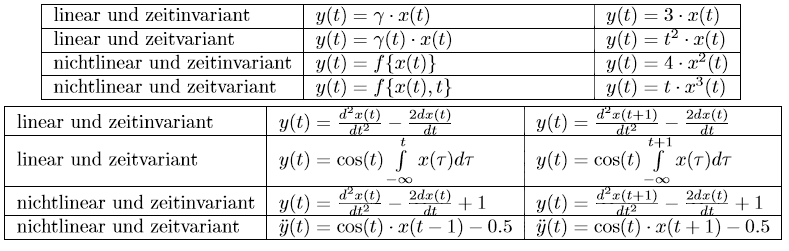
\includegraphics[width=\columnwidth]{Images/system_beispiele}


\subsection{Stabilität}
\textbf{BIBO-Stabilität}\\
\script{177} BIBO-stabil bedeutet, wenn beschränktes Eingangssignal ein beschränktes Ausgangssignal ergibt.
\[
\int_{-\infty}^{\infty}\left|h(t)\right|dt < \infty
\]

Beispiel: $y(t) = e^tx(t)$ ist instabel, linear und zeitvarient. $y(t)t = \frac{x^4(t)}{1000}$ ist BIBO-stabil, nicht linear und zeitvariant.
\\ ~\\
\textbf{Asymptotische Stabilität}\\ \script{178}
Ein LTI-System ist asymptotisch stabil, wenn seine Impulsantwort asymptotische gegen Null abklingt d.H. $\lim\limits_{t\rightarrow\infty}h(t) = 0$. Dabei sind passive Netzwerk immer stabil.

\begin{center}
\includegraphics[width=0.4\columnwidth]{Images/stabilität}
\end{center}

\noindent\underline{Instabil}: Wenn mindestens ein Pol in der Rechten s-Halbebene liegt oder wenn ein mehrfach Pol (zB $\frac{1}{(s^2 + 1)^2} \rightarrow \pm j$) auf der j-Achse liegt.\\
\underline{Grenzstabilität}: Wenn kein Pol in der rechten s-Halbebene liegt und kein mehrfach Pol und mindestens ein einfacher Pol auf der j-Achse liegt.\\
\underline{Stabil:} Pol nur in der linken s-Halbebene.\\

~\\
Die Stabilität eines Polynom $P(s) = a_ns^n + a_{n-1}s^{n-1}+a_1s + a_0$ kann auch durch die \textbf{Hurwitz-Kriterium} überprüft werden. 
\underline{stabil}: alle Koeffizienten $a_i > 0$ für $i \in [0;n]$ und die Hurwitz-Determinante $D_i > 0$ für $i\in[1;n]$.

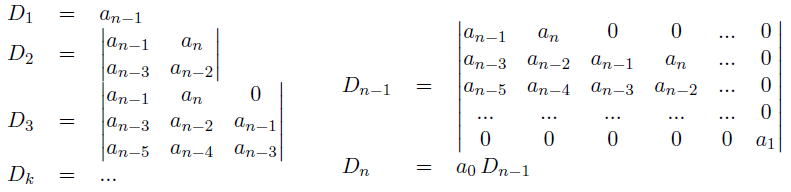
\includegraphics[width=\columnwidth]{Images/hurwitz}
\\ ~\\
\textbf{Beispiel}:
\[
H(s) = \frac{Y(s)}{X(s)} = \frac{3s^2 + 14s + 14}{s^3 + 17s^2 + 14s + 8}
\]
Das bedeutet $n=3$, $a_3 = 1, a_2=17, a_1 = 14, a_0=8$. 
\begin{align*}
	D_1 &= a_2 > 0 \\
	D_2 &= \begin{vmatrix*} a_2 & a_3 \\ a_0 & a_1 \end{vmatrix*} = 17\cdot 14 - 1\cdot 8 > 0 \\
	D_3 &= \begin{vmatrix*} a_2 & a_3 & 0 \\ a_0 & a_1 & a_3 \\ 0 & 0 & a_0	\end{vmatrix*} > 0
\end{align*}

Dieses LTI-System ist \underline{Stabil}

\subsection{Phasen- und Gruppenlaufzeiten}\script{182}
Verzögerung eines Signals durch ein System sind definiert durch Phasenlaufzeit für ein einzelnes bzw. Gruppenlaufzeit für mehrere Sinusschwingungen.

\noindent\textbf{Phasenlaufzeit}
\[
\tau_P(\omega) = \frac{-\theta(\omega)}{\omega}
\]

\noindent\textbf{Gruppenlaufzeit}
\[
\tau_G(\omega) = \frac{-d\theta(\omega)}{d\omega}
\]

\textbf{Beispiel:} Gruppen- und Phasenlaufzeit eines AM-Signals $x(t) = (1+0.8\sin(0.05t))\sin(t)$ wird durch das System $H(s) \frac{1}{s^2 + 0.2s + 1} = \frac{1}{(1 -\omega^2) + 0.2\omega j}$ übertragen.\\
Der Amplitudengang $|H(jw)| = \frac{1}{\sqrt{(1-\omega^2)^2 + (0.2\omega)^2}}$. Daraus kann die Phase berechnet werden $\theta(\omega) = -\arctan\left(\frac{0.2\omega}{1-\omega^2}\right)$, was schliesslich zur Phasenlaufzeit führt.
\begin{align*}
	\tau_P(\omega) &= \frac{-\theta(\omega)}{\omega} \rightarrow \frac{-(-\arctan\left(\frac{0.2\omega}{1-\omega^2}\right))}{\omega} \\
	&= \frac{\arctan\left(\frac{0.2\omega}{1-\omega^2}\right)}{\omega} 
\end{align*}

Die Gruppenlaufzeit kann durch Ableiten von $\frac{-d\theta(\omega)}{d\omega}$ bestimmt werden
\begin{align*}
	\tau_G(\omega) &= \frac{-d\theta(\omega)}{d\omega} \xRightarrow[= \frac{1}{1+x^2}]{\arctan'(x)} \frac{-1}{1 + \left(\frac{0.2\omega}{1 - \omega^2}\right)^2} \cdot \overbrace{\frac{0.2(1-\omega^2) + 0.4\omega^2}{(1 - \omega^2)^2}}^\text{Innere Ableitung} \\
	&= -\frac{0.2(1+\omega^2)}{1-1.96\omega^2 + \omega^4}
\end{align*}


Die Verschiebung kann mit $\omega = 1$ (weil Trägersignal $\sin(1\cdot t)$ ist) bestimmt werden:
\begin{align*}
	\left.\tau_G(\omega)\right|_{\omega = 1} &= -10s \\
	\left.\tau_P(\omega)\right|_{\omega = 1} &= 1.5s 
\end{align*}
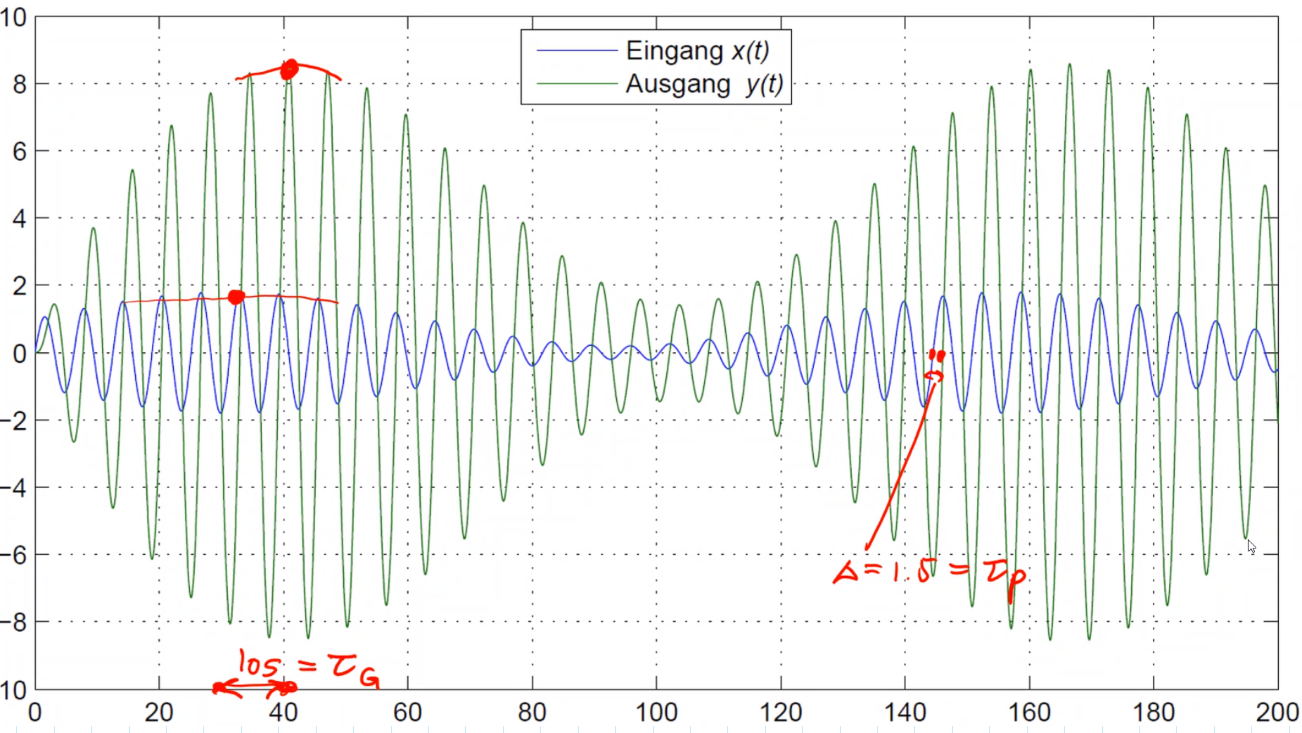
\includegraphics[width=\columnwidth]{Images/gruppenlaufzeit}


\subsection{Verzerrung}\script{189}
\textbf{Klirrfaktor} $k$ ist definiert als Verhältnis des Effektivwerts der neu am Ausgang eines Systems einstandenen Harmonischen Oberschwingungen ($U_2, U_3$) zum Effektivwert des gesamten Signals:
\[
k = \sqrt{\frac{U^2_2 + U^2_3 + \dots + U_n^2}{U^2_1 + U^2_3 + \dots + U_n^2}}
\]
Er Beschreibt die nichtlinearen Verzerrungen eines Systems.

\subsection{Kaskadierung}
Serien-Schaltungen werden multipliziert (Matlab: \textit{series(s1, s2)}). Parallel-Schaltung werden addiert/subtrahiert (Matlab: \textit{parallel(s1, s2)}). Rückkopplung nur mit (Matlab: \textit{feedback(s1, s2,+1)})
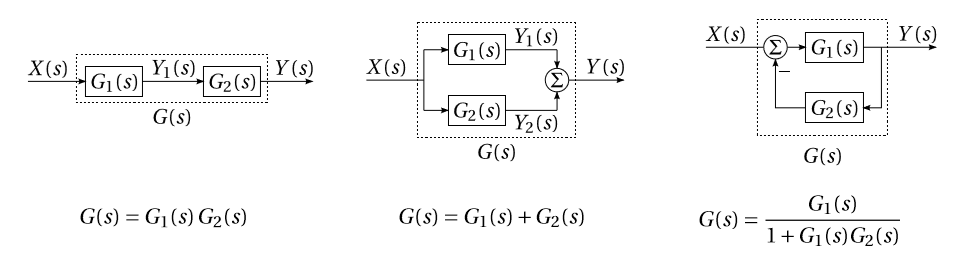
\includegraphics[width=\columnwidth]{Images/systeme}

\subsection{Übertragung von stochastischen Signalen}
\script{193}
Bei stochastischen Signalen können nur Leistungen berechnet werden, da das Signal $x(t)$ zufällig ist. Die Kreuzkorrelationsfunktion $\varphi_{xy}(\tau)$ eines stochastischen Signals ist
\[
\varphi_{xy}(\tau) = h(\tau)*\varphi_{xx}(\tau) \transform \varPhi(j\omega) = H(j\omega)\cdot\varPhi(j\omega)
\]

\noindent Die Leistungsdichtespektrum $\varPhi_{yy}(j\omega)$ vom stochastischen Signal $x$
\[
\varPhi_{yy}(j\omega) = \left|H(j\omega)\right|^2\varPhi_{xx}(j\omega)
\]
kann durch Rücktransformation die Leistung von $y$ erhalten werden
\begin{align*}
	\varPhi_{yy}(j\omega) &\itransform \varphi_{yy}(\tau) \\
	\varphi_{yy}(\tau) &= \frac{1}{2\pi}\int_{-\infty}^{\infty}\left|H(j\omega)\right|^2\varPhi_{xx}(j\omega)e^{j\omega\tau}d\omega\\
	Y^2 = \varphi_{yy}(0) &= \frac{1}{2\pi}\int_{-\infty}^{\infty}\left|H(j\omega)\right|^2\varPhi_{xx}(j\omega)d\omega
\end{align*}
